\documentclass[11pt,a4paper]{article}

\usepackage[margin=1in]{geometry}
\usepackage{amsmath,amssymb}
\usepackage{booktabs}
\usepackage{tabularx}
\usepackage{array}
\usepackage{graphicx}
\usepackage{caption}
\usepackage{subcaption}
\usepackage{siunitx}
\usepackage{hyperref}
\usepackage{microtype}

\graphicspath{{../../}}
\sisetup{detect-all}

\hypersetup{
  colorlinks=true,
  linkcolor=black,
  citecolor=black,
  urlcolor=blue
}

\newcommand{\method}{S2R-FocusNet}

\title{Simulation-to-Real Focus-Stack Reconstruction for Reflective Surface Defect Morphology Using Prior-Guided Deep Correction}
\author{Li Shenshi \and Qian Fengfan}
\date{}

\begin{document}

\maketitle

\begin{abstract}
Reflective industrial surface defects require three-dimensional morphology reconstruction to characterize local depth variations, boundary structures, and micro-scale surface irregularities that are difficult to describe from two-dimensional images alone. However, calibrated height ground truth is difficult to obtain for real microscopic reflective surfaces, which limits the direct training and quantitative evaluation of learning-based reconstruction methods. To address this data bottleneck, this work studies a simulation-to-real focus-stack reconstruction framework for reflective surface defect morphology. The framework uses controllable synthetic focus stacks with known height maps for supervised training and quantitative evaluation, and combines traditional depth-from-focus priors, glare-aware focus cues, focal-difference representation, and a compact learning-based correction model. On the current synthetic test set, the proposed Focus-ResUNet implementation achieves the lowest mean absolute error among the evaluated internal classical and learning-based baselines, with a mean MAE of \SI{53.22}{\micro\meter} and an edge MAE of \SI{86.68}{\micro\meter}. On real focus-stack samples without calibrated height ground truth, no-reference morphology metrics show reduced low-confidence spike artifacts and improved reconstruction stability compared with direct DFF-based methods. The results suggest that prior-guided correction over simulation-derived supervision is a practical route for relative morphology reconstruction of reflective surface defects, while calibrated real-height validation and broader external deep DFF comparisons remain important future work.
\end{abstract}

\noindent\textbf{Keywords:} depth from focus; focus stack; reflective surface defect; simulation-to-real; morphology reconstruction; prior-guided learning

\section{Introduction}

Industrial surface inspection has increasingly relied on image-based methods for detecting scratches, pits, dents, holes, local steps, and texture anomalies. Two-dimensional images are effective for locating visible defects, yet many inspection tasks also require a structural description of local depth variation, boundary continuity, and micro-scale surface morphology. This requirement is especially important for reflective surfaces, where intensity is affected by illumination, specular highlight, surface roughness, and local geometry. Recovering three-dimensional morphology from microscopic focus-stack sequences is therefore a useful step toward defect characterization beyond visual detection alone.

Shape from focus and depth from focus (DFF) infer height from the change of image sharpness across a sequence captured at different focal positions. Classical focus-based reconstruction is attractive because it is interpretable, does not require large annotated datasets, and can be built on ordinary microscope imaging sequences. However, the reliability of the estimated height map strongly depends on the focus measure and local support window. Weak texture, periodic texture, glare, saturated highlights, sharp defect edges, and multi-peak focus responses can produce incorrect focal-layer selection and unstable height spikes. Adaptive-window methods reduce part of this ambiguity, but reflective microscopic surfaces remain difficult when the focus cue itself is unreliable.

The central bottleneck addressed in this work is the scarcity of calibrated real height ground truth. Profilometer, confocal, interferometric, or calibrated step-height measurements can provide accurate references, but they may be costly, slow, unavailable, or hard to synchronize with every real focus-stack sample. Direct supervised learning on real microscopic reflective defects is therefore difficult. We adopt a simulation-to-real strategy: synthetic surfaces are generated with known height maps, rendered into focus stacks under controlled geometry, roughness, reflectance, focal sampling, and glare-related conditions, and then used for supervised training and absolute quantitative evaluation. Real focus stacks are used separately for no-reference morphology validation.

This paper studies a prior-guided focus-stack correction framework, denoted as \method. Instead of treating the raw focus stack as the only input, the framework combines traditional DFF and glare-aware DFF (GADFF) priors, focal-difference features, glare or high-risk cues, and a compact encoder-decoder correction network. The focus-based priors provide interpretable axial estimates, while the learning component corrects unstable local artifacts and improves morphology continuity under limited training data. This design is intended to reduce the learning burden and preserve the physical cues embedded in the focal sequence.

The main contributions of this draft are as follows.
\begin{enumerate}
  \item We construct a controllable synthetic focus-stack dataset for reflective defect morphology, where each sample has a known height map for quantitative evaluation.
  \item We formulate reflective surface reconstruction as prior-guided focus-stack correction, combining DFF/GADFF priors, focal-difference representation, glare-aware cues, and learning-based height correction.
  \item We establish a two-level evaluation protocol that separates synthetic absolute height-error evaluation from real no-reference morphology validation.
  \item We report current internal comparison results and identify the remaining submission-critical gaps, including external deep DFF baselines, module ablation, and calibrated real-height validation.
\end{enumerate}

\begin{figure}[t]
  \centering
  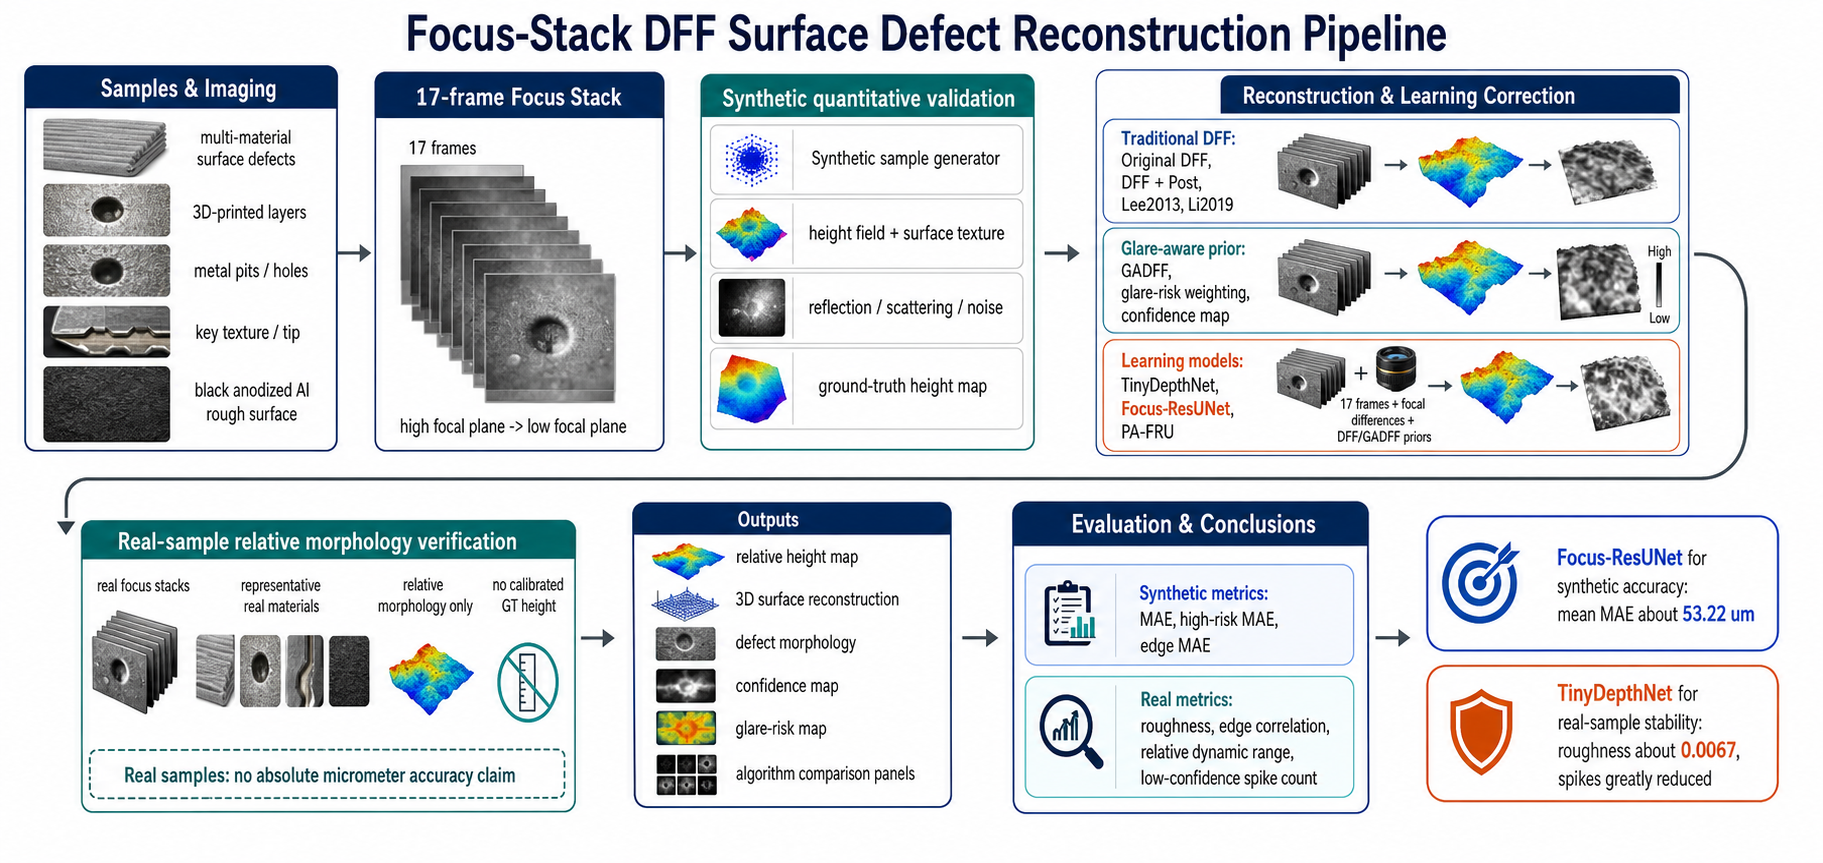
\includegraphics[width=\linewidth]{output/imagegen/focus_stack_dff_pipeline_v2.png}
  \caption{Overview of the simulation-to-real focus-stack reconstruction pipeline. Synthetic surfaces with known height maps are rendered into focus stacks for supervised training, while DFF/GADFF priors and focal-difference representations provide interpretable axial cues. Real focus stacks are evaluated with no-reference morphology metrics because calibrated real height ground truth is unavailable.}
  \label{fig:pipeline}
\end{figure}

\section{Related Work}

\subsection{Classical Shape and Depth from Focus}

Classical shape from focus estimates depth by locating the focal position with the strongest local sharpness response. Nayar and Nakagawa established the feasibility of focus-based shape recovery, and later work analyzed focus-measure operators such as gradient, Laplacian, variance, and frequency-domain responses \cite{nayar_shape_1994,pertuz_analysis_2013}. These methods are attractive in microscopy and industrial inspection because they provide an interpretable connection between optical focus response and estimated depth. Their limitations arise when local texture is weak, the support window is poorly matched to the structure scale, or glare distorts the measured sharpness response.

Adaptive-window strategies address part of this problem by changing the support region according to local image structure. Lee et al. proposed adaptive window selection for 3D shape recovery from image focus, while Li et al. introduced an adaptive window iteration algorithm for enhanced focus-based reconstruction \cite{lee_adaptive_2013,li_adaptive_2019}. In this project, these approaches serve as stronger classical baselines than a simple fixed-window DFF pipeline.

\subsection{Learning-Based Depth from Focus}

Learning-based DFF methods replace handcrafted focus selection with trainable models that can aggregate spatial and focal information. DDFFNet was among the early end-to-end deep DFF methods and showed that learning can substantially improve focus-stack depth estimation when calibrated training data are available \cite{jawahar_deep_2019}. AiFDepthNet further connected depth prediction with all-in-focus supervision, which is relevant when depth labels are incomplete or unavailable \cite{wang_bridging_2021}.

DFV is especially relevant to this work because it explicitly models differential focus information along the focal dimension \cite{yang_deep_2022}. Our focal-difference representation follows the same broad observation: depth cues are encoded not only in individual focused frames but also in how local features change between neighboring focal planes. More recent learning-based focus-stack methods also address real-camera adaptation, camera-setting invariance, and robustness to synthetic-to-real gaps, including DfF in the Wild and DDFS \cite{won_learning_2022,fujimura_deep_2024}. These methods are important external baselines for future experiments.

\subsection{Simulation-to-Real and Defocus-Based Learning}

The lack of calibrated real height maps has motivated simulation, defocus modeling, and self-supervised learning strategies. Focus on Defocus used defocus cues to bridge synthetic and real domains for depth estimation \cite{maximov_focus_2020}. DEReD explored fully self-supervised depth estimation from defocus clues, showing that optical reconstruction constraints can be useful when dense depth labels are unavailable \cite{si_fully_2023}. These directions support the present project's data strategy: synthetic focus stacks provide controlled height supervision, while real stacks can be used for no-reference validation and later self-training.

Recent monocular foundation depth models provide a complementary perspective. Depth Anything V2 shows that replacing noisy labeled real depth with precise synthetic labels, scaling the teacher model, and using large-scale pseudo-labeled real images can improve monocular depth generalization \cite{depth_anything_v2_2024}. This is relevant to our simulation-to-real story as a training-strategy reference and as a possible source of single-frame relative-depth priors. However, monocular depth models process single images and do not use the axial focus response of a focal stack, so they should be treated as auxiliary references rather than direct DFF baselines in the main quantitative table.

\subsection{Industrial Surface Morphology Reconstruction}

Industrial surface defect research has often emphasized two-dimensional detection and classification, but defect severity is frequently related to three-dimensional morphology, such as pit depth, edge collapse, scratches, burrs, and local roughness \cite{ren_surface_2021}. Recent work on microscopy and structured illumination reconstruction also highlights the value of 3D morphology for defect characterization \cite{wang_defect_2026}. The present work is positioned in this transition from visual defect localization to relative morphology reconstruction for reflective microscopic surfaces.

\section{Method}

\subsection{Problem Formulation}

Let \(I=\{I_1,\ldots,I_N\}\) denote an \(N\)-frame focus stack captured at different focal positions \(z=\{z_1,\ldots,z_N\}\). The goal is to estimate a relative surface height map \(H\) from the focus-stack observations. For synthetic samples, the ground-truth height map \(H^\ast\) is available for supervised training and quantitative evaluation. For real samples, calibrated height ground truth is unavailable, and evaluation is restricted to no-reference morphology indicators.

The proposed framework estimates height using both image observations and focus-based priors:
\begin{equation}
\hat{H}=f_{\theta}(I, P_{\mathrm{DFF}}, P_{\mathrm{GADFF}}, D_{\mathrm{focal}}, M_{\mathrm{risk}}),
\end{equation}
where \(P_{\mathrm{DFF}}\) is the traditional DFF prior, \(P_{\mathrm{GADFF}}\) is the glare-aware DFF prior, \(D_{\mathrm{focal}}\) denotes focal-difference features, and \(M_{\mathrm{risk}}\) denotes glare or high-risk cues when available. In the current implementation files, the main learning model is reported as Focus-ResUNet; in this manuscript draft it is unified under the working name \method.

\subsection{Synthetic Focus-Stack Data Construction}

Synthetic data is the controlled source of height ground truth. The current dataset contains 12 training samples, 5 validation samples, and 7 test samples. Each sample contains 17 focus-stack layers and a known height map. The test set covers V-valley, ridge, mountain, step, periodic stripe, and pit or groove structures, with depth ranges from \SI{920}{\micro\meter} to \SI{1420}{\micro\meter}. This controlled setting enables absolute metrics such as MAE, edge MAE, and high-risk-region MAE.

The simulation is designed around six factors: surface geometry, surface texture and roughness, axial sampling, height range, reflectance and glare disturbance, and rendered focus response. Procedural geometry and noise patterns are used to generate height fields; focus-stack frames are rendered across focal layers; and glare/high-risk cues are estimated from highlight and instability patterns. These synthetic factors make the data generator a central component of the simulation-to-real research strategy.

\begin{table}[t]
  \centering
  \caption{Current synthetic dataset split. Each sample contains a 17-layer focus stack and a known height map.}
  \label{tab:dataset_split}
  \small
  \begin{tabularx}{\linewidth}{lccX}
    \toprule
    Split & Samples & Stack layers & Role \\
    \midrule
    Train & 12 & 17 & Supervised training with known synthetic height maps \\
    Validation & 5 & 17 & Model selection and parameter checking \\
    Test & 7 & 17 & Quantitative evaluation on held-out synthetic geometries \\
    \bottomrule
  \end{tabularx}
\end{table}

\subsection{Focus-Based Priors}

Traditional focus-based estimates are used in two roles. First, Original DFF, DFF with post-processing, Lee2013, Li2019, and GADFF define interpretable baselines. Second, DFF/GADFF-related outputs provide physically meaningful axial cues for the learning-based correction network. This prior-guided design is intended to make the network correct failure cases around weak texture, glare, and sharp boundaries instead of learning the full focus-depth relation only from raw image stacks.

It is important to distinguish prior usefulness from standalone accuracy. The current synthetic results show that GADFF is unstable when used alone, but it can still contribute glare-aware information as an auxiliary cue. The final paper should strengthen this claim with ablation experiments that remove each prior channel.

\subsection{Focal-Difference Representation}

Focus-stack depth information is encoded across the focal dimension. Therefore, the framework uses focal-difference features to represent how image or focus responses change between neighboring focal positions. This representation is motivated by the same principle behind DFV: first-order variation along the focal sequence can make the network sensitive to focus transitions and local depth cues. In the current draft, the exact implementation of the difference operator should be verified from the training code before final submission.

\subsection{Prior-Guided Correction Network}

\begin{figure}[t]
  \centering
  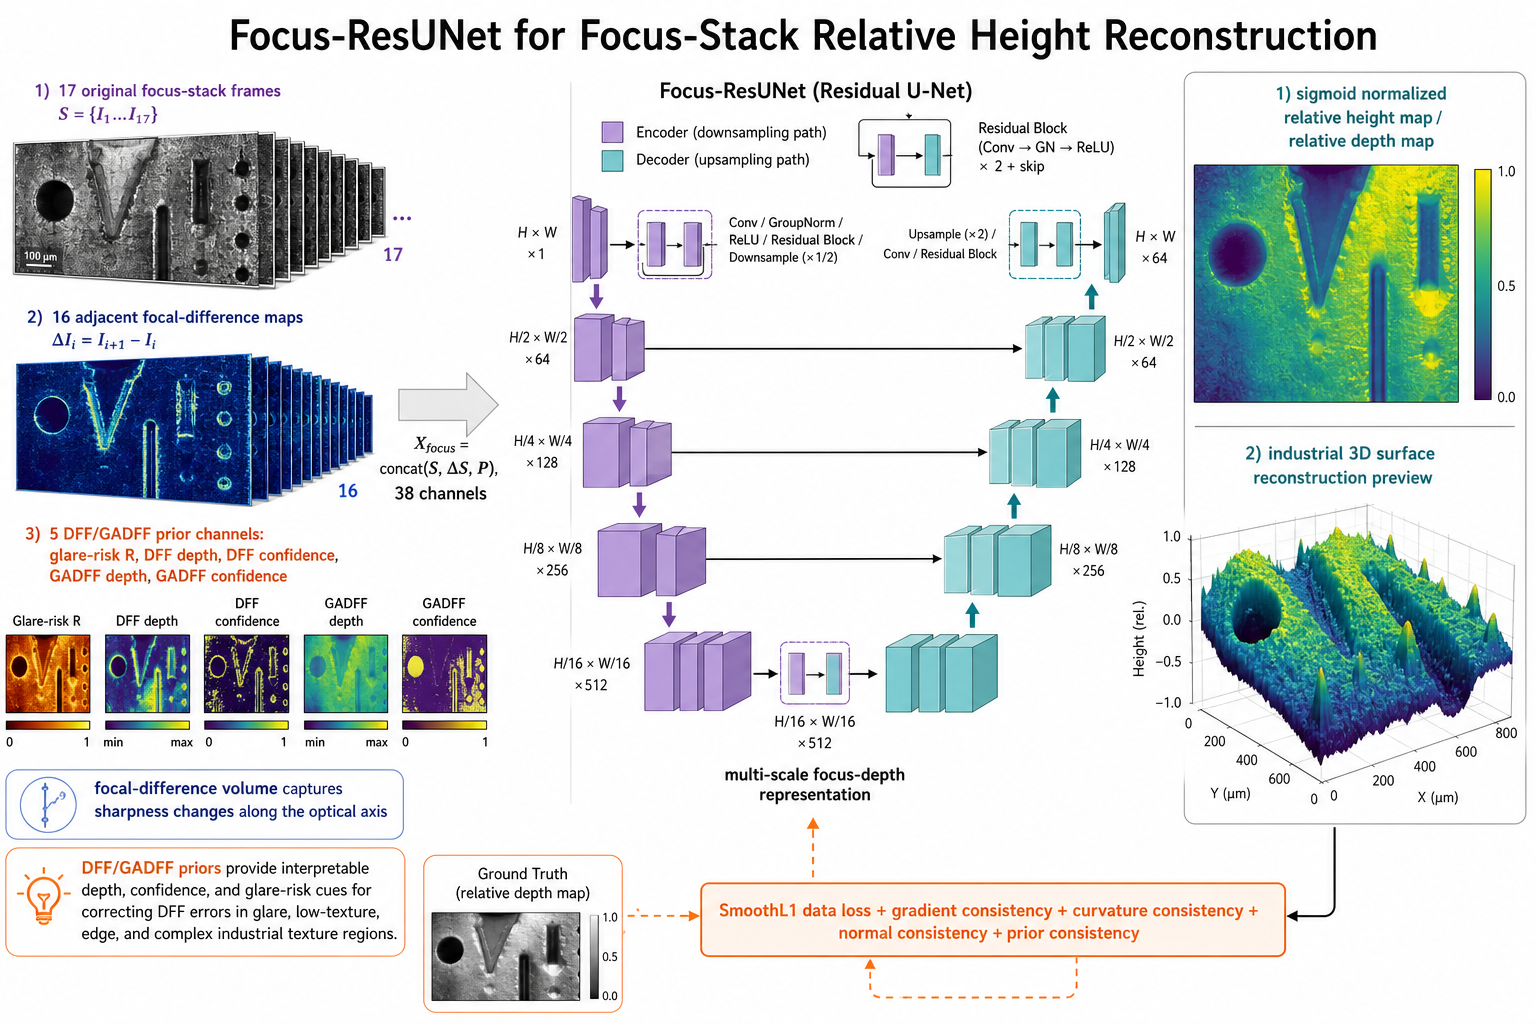
\includegraphics[width=\linewidth]{output/imagegen/focus-resunet-industrial-network-diagram-final-2048x1152.png}
  \caption{Architecture of the prior-guided focus-stack correction network. The model integrates raw focus-stack information, DFF/GADFF priors, focal-difference features, and glare-aware cues to predict a corrected height map while preserving focus-based physical cues.}
  \label{fig:architecture}
\end{figure}

The correction network uses a ResUNet-style encoder-decoder backbone to combine local image evidence with prior height cues. Encoder features aggregate local texture, focus, and prior information, while decoder features reconstruct a dense height map. Skip connections help preserve spatial detail around defect edges. The model is compact relative to large generic depth networks, which is appropriate for the current limited synthetic training set.

The manuscript should treat TinyDepthNet, Focus-ResUNet, and residual Focus-ResUNet as internal variants or baselines. The final contribution should be written as one method, \method, with the best verified implementation selected for submission.

\subsection{Training and Inference}

For synthetic samples, the network is trained with known height maps. The current safe description is supervised height reconstruction; any edge-aware, high-risk weighted, smoothness, residual-bound, or prior-consistency losses should only be written as implemented method components after code verification. Otherwise, they should remain as future extensions or ablation candidates.

During inference, the trained model receives real focus stacks and corresponding focus-based priors, then outputs a relative morphology map. Because calibrated real height maps are unavailable, real-sample evaluation uses no-reference morphology metrics, including roughness stability, edge retention, relative dynamic range, and low-confidence spike count. These metrics indicate output stability and morphology plausibility, not calibrated geometric accuracy.

\section{Experiments}

\subsection{Evaluation Protocol}

The experiments are organized into two evidence chains. The synthetic test set supports absolute quantitative evaluation because height maps are known. The real focus-stack set supports deployment-oriented morphology validation under no-reference evaluation because calibrated real height ground truth is unavailable. This separation is essential for avoiding overstatement of real-sample accuracy.

\subsection{Baselines and Metrics}

The current internal baselines include Original DFF, DFF with post-processing, GADFF, Lee2013 adaptive-window DFF, Li2019 adaptive-window iteration, TinyDepthNet, Focus-ResUNet, and residual Focus-ResUNet. External deep DFF baselines such as DDFFNet and DFV are identified as priority additions, but their results are not yet reported in this draft.

For synthetic samples, the main metrics are mean absolute error (MAE), edge MAE, and high-risk MAE in micrometers. Edge MAE evaluates defect boundaries and discontinuities, while high-risk MAE focuses on glare, weak-texture, or otherwise unstable regions. For real samples, the metrics are no-reference indicators: roughness, edge retention, relative dynamic range, and low-confidence spike count.

\subsection{Synthetic Quantitative Results}

\begin{figure}[t]
  \centering
  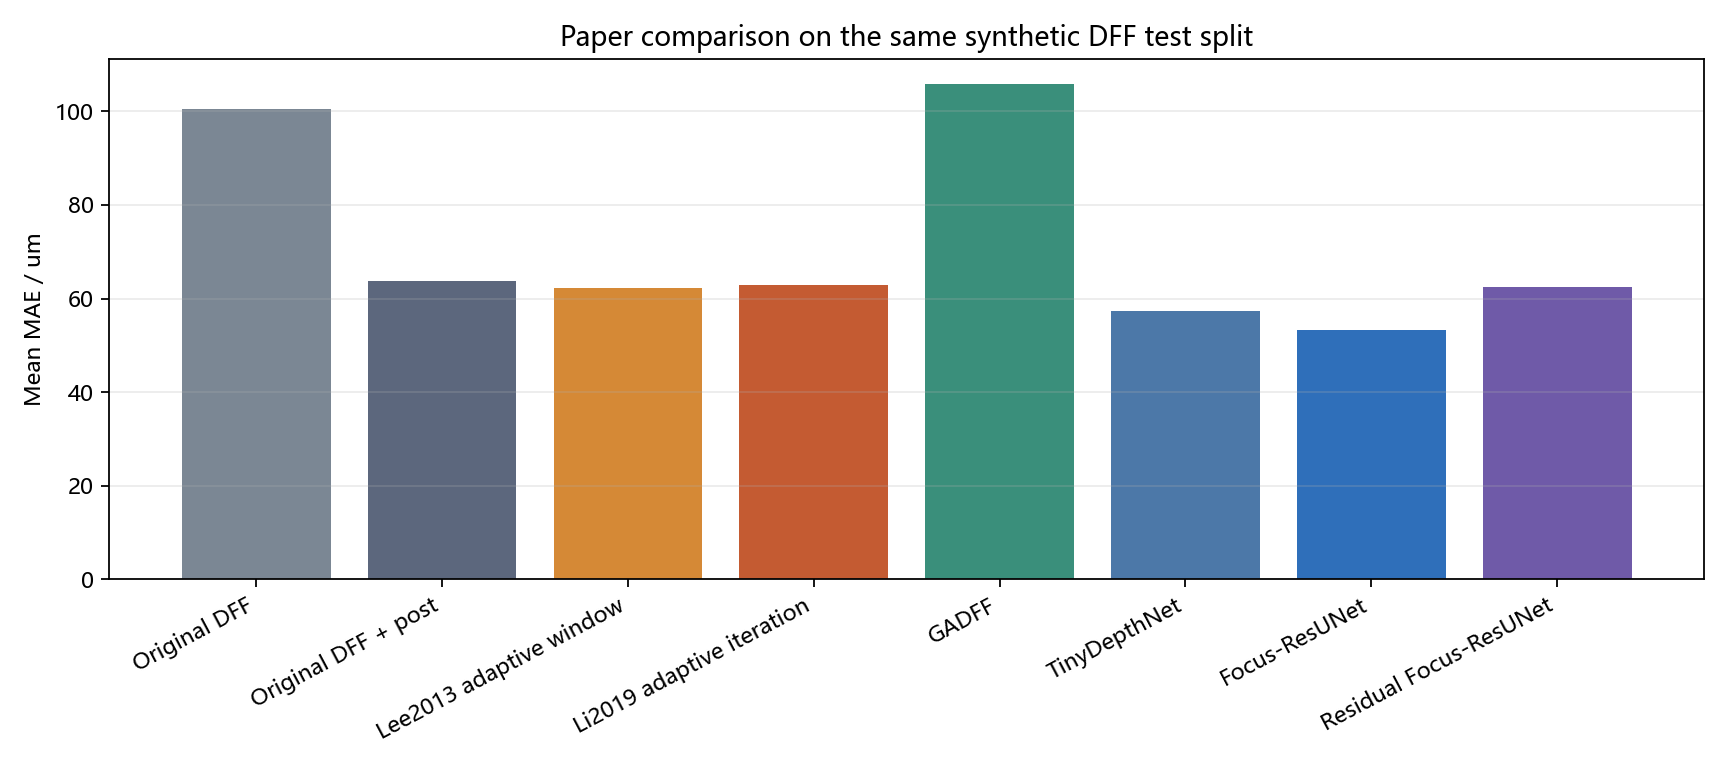
\includegraphics[width=.82\linewidth]{results/figures/paper_comparison_mean_mae.png}
  \caption{Synthetic quantitative comparison based on the current internal baselines. Focus-ResUNet achieves the lowest mean MAE among the evaluated internal methods, while high-risk regions remain a key limitation to analyze in later ablation and failure studies.}
  \label{fig:synthetic_results}
\end{figure}

\begin{table}[t]
  \centering
  \caption{Mean synthetic test-set metrics for the current internal methods. Lower is better. External DFV and DDFFNet results are planned but not yet included.}
  \label{tab:synthetic_comparison}
  \small
  \begin{tabular}{lrrr}
    \toprule
    Method & Mean MAE ($\mu$m) & Edge MAE ($\mu$m) & High-risk MAE ($\mu$m) \\
    \midrule
    Focus-ResUNet & 53.22 & 86.68 & 40.14 \\
    TinyDepthNet & 57.31 & 89.10 & 42.63 \\
    Lee2013 adaptive window & 62.35 & 146.83 & 30.52 \\
    Residual Focus-ResUNet & 62.52 & 126.91 & 30.08 \\
    Li2019 adaptive iteration & 62.95 & 145.33 & 31.24 \\
    DFF + post-processing & 63.81 & 149.04 & 29.72 \\
    Original DFF & 100.55 & 206.61 & 46.32 \\
    GADFF & 105.83 & 210.60 & 46.38 \\
    \bottomrule
  \end{tabular}
\end{table}

On the current seven-sample synthetic test set, Focus-ResUNet achieves the lowest mean MAE and edge MAE among the evaluated internal baselines. This result supports the value of learning-based correction for overall morphology reconstruction and edge stability under the current synthetic protocol. However, the high-risk MAE is not the lowest among all methods. This indicates that reflective glare, weak texture, and locally ambiguous focus responses remain difficult and require more targeted modeling.

\subsection{Real No-Reference Morphology Evaluation}

\begin{figure}[t]
  \centering
  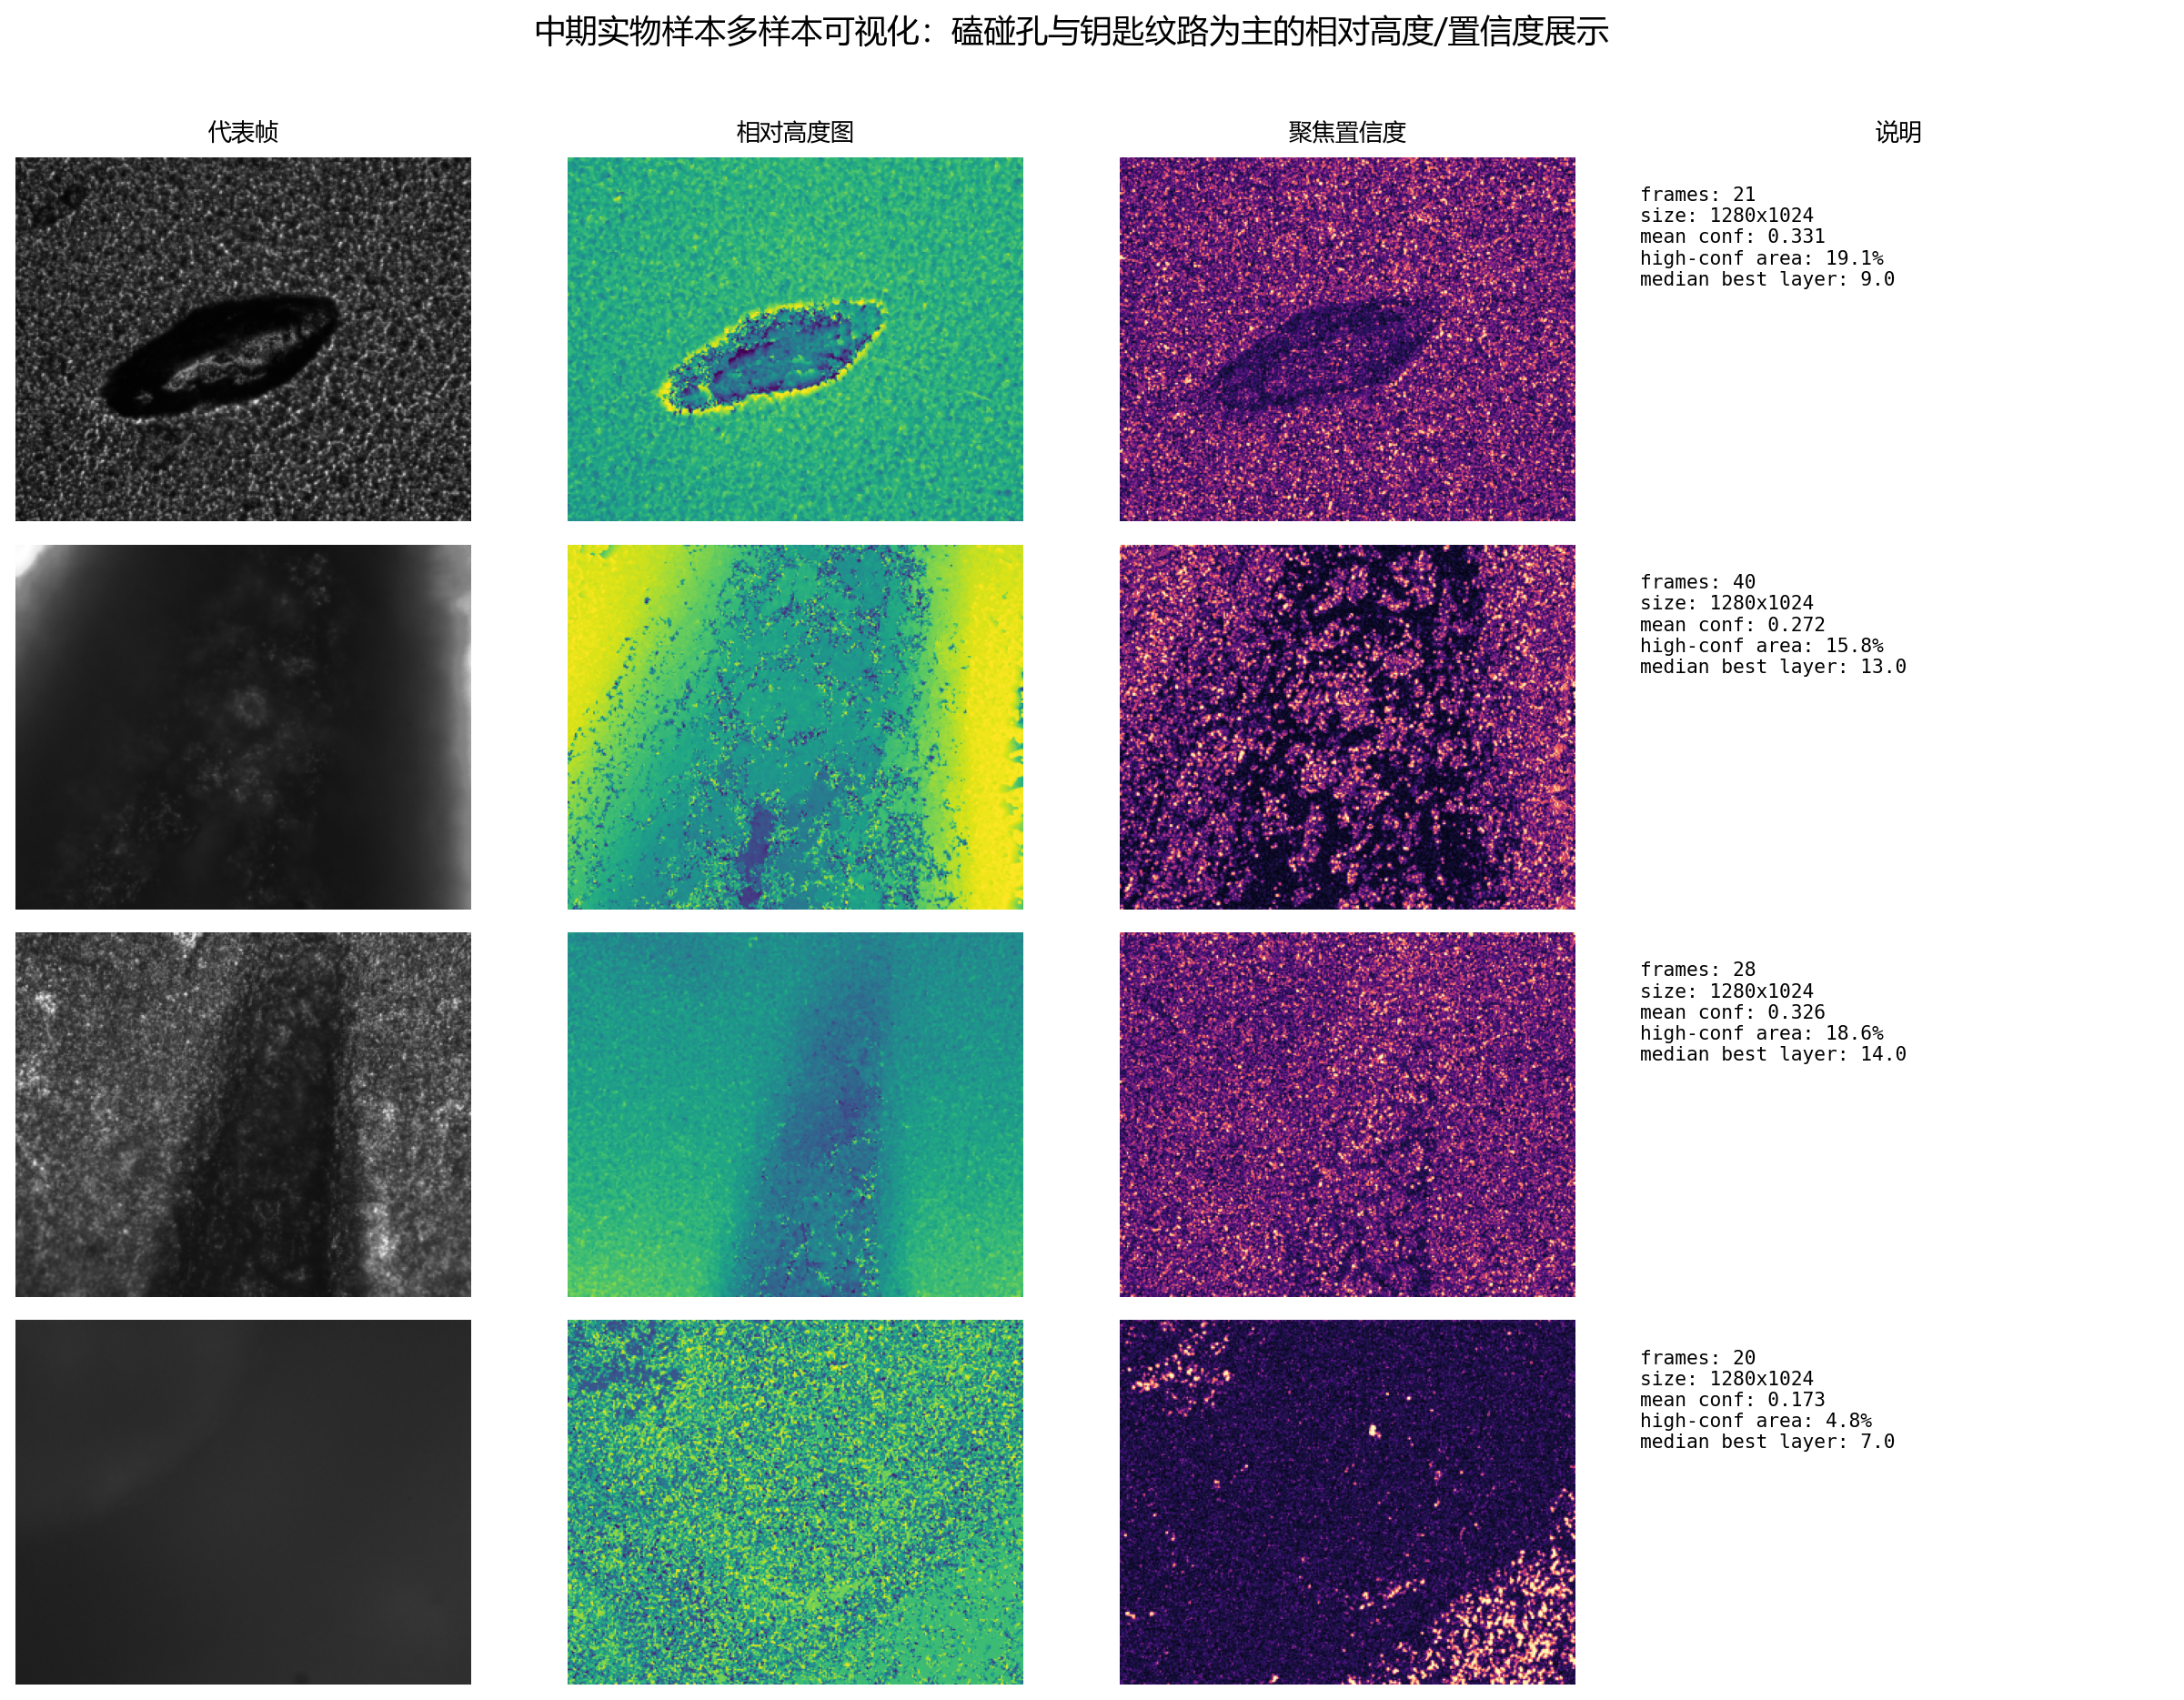
\includegraphics[width=\linewidth]{results/figures/real_midterm_multisample_panel.png}
  \caption{Real focus-stack reconstruction results under no-reference evaluation. Since calibrated real height ground truth is unavailable, the comparison focuses on morphology stability, relative dynamic range, and low-confidence spike suppression rather than absolute height accuracy.}
  \label{fig:real_results}
\end{figure}

\begin{table}[t]
  \centering
  \caption{Real no-reference morphology metrics. These metrics should be interpreted as stability and plausibility indicators rather than calibrated height accuracy.}
  \label{tab:real_metrics}
  \small
  \begin{tabular}{lrrrr}
    \toprule
    Method & Roughness & Edge retention & Dynamic range & Spike count \\
    \midrule
    Focus-ResUNet & 0.0078 & 0.0009 & 0.5317 & 2.0 \\
    TinyDepthNet & 0.0067 & -0.0243 & 0.3623 & 49.0 \\
    DFF + post-processing & 0.0130 & -0.0296 & 0.3944 & 4091.3 \\
    GADFF & 0.0316 & -0.0295 & 0.5406 & 3351.4 \\
    Lee2013 adaptive window & 0.0295 & -0.0209 & 0.6325 & 5018.7 \\
    Li2019 adaptive iteration & 0.0318 & -0.0233 & 0.6515 & 5433.6 \\
    Original DFF & 0.0977 & -0.0394 & 0.6964 & 9179.7 \\
    Residual Focus-ResUNet & 0.0594 & -0.0343 & 0.5203 & 9262.1 \\
    \bottomrule
  \end{tabular}
\end{table}

On real focus-stack samples, Focus-ResUNet substantially reduces low-confidence spike artifacts compared with direct DFF-based methods. The result supports morphology stability under no-reference evaluation. It does not establish absolute real-world height accuracy because calibrated real height maps are not available.

\subsection{External Baseline and Ablation Plan}

The current draft does not claim superiority over external SOTA methods. DFV and DDFFNet are the priority external deep DFF baselines because they directly process focal stacks and provide stronger comparison with learning-based focus-stack reconstruction. DFV is especially important because its differential focus volume is closely related to the focal-difference representation used here. Future experiments should use a unified synthetic split, frame-count protocol, output-scale alignment rule, and MAE/edge-MAE/high-risk-MAE metrics.

Depth Anything V2 is handled through a separate auxiliary protocol. If it is used, the input should be a single frame selected from the focus stack, such as a center-focus frame, a focus-measure-selected best-focus frame, or an all-in-focus fusion image. The output should be reported as monocular relative depth for qualitative comparison or as a scale-aligned synthetic sanity check kept outside the main SOTA table. This protocol allows the paper to discuss foundation-depth priors and pseudo-label training strategies without mixing single-image monocular depth with focus-stack baselines.

The minimum ablation set should include:
\begin{itemize}
  \item the full \method;
  \item a version without DFF and GADFF priors;
  \item a version without focal-difference representation;
  \item a version without glare-aware cues;
  \item a direct image-to-depth variant as a lower-prior learning baseline.
\end{itemize}
These experiments are needed before making strong claims about the independent contribution of each module.

\section{Discussion}

\subsection{Role of Simulation-Based Supervision}

The synthetic focus-stack dataset plays a central role because it provides known height maps for supervised training and absolute quantitative evaluation. For reflective microscopic surfaces, collecting calibrated real height ground truth for every defect sample is difficult, especially when local glare, surface roughness, and micro-scale morphology interact with the imaging process. Simulation makes it possible to control surface geometry, roughness, depth range, focal sampling, and glare-related factors independently. This supports controlled analysis under known conditions while keeping real-sample claims limited to no-reference validation.

\subsection{Effect of Prior-Guided Correction}

The current internal results suggest that learning-based correction can improve overall reconstruction accuracy and edge stability on the synthetic test set. Classical DFF is interpretable but sensitive to weak texture, glare, and boundary ambiguity. A direct image-to-depth model may require more data to learn focus geometry reliably. Prior-guided correction provides a practical compromise: traditional focus-based estimates serve as physical anchors, and the network focuses on local correction and morphology continuity. Stronger claims about each prior module require ablation.

\subsection{Limitations of Real-Sample Evaluation}

Real-sample results should be interpreted carefully. The reduced spike count and improved stability indicate that the model suppresses some unstable focus responses when applied outside the synthetic domain. However, without calibrated real height maps, the real metrics do not measure absolute geometric accuracy. A small calibrated real subset, such as step-height, profilometer, confocal, or interferometric measurements, would substantially strengthen the final manuscript.

\subsection{High-Risk Reflective Regions}

Although the current model achieves the lowest synthetic mean MAE and edge MAE among internal baselines, high-risk MAE remains weaker than several traditional or residual variants. This result suggests that glare, weak texture, and ambiguous focus responses need targeted modeling. Future versions should consider high-risk weighted losses, confidence calibration, explicit glare-region modeling, and profile-based failure analysis.

\subsection{Relation to Foundation Depth Models}

Depth Anything V2 and related monocular foundation models are valuable for understanding large-scale data and pseudo-label training strategies. Their use of precise synthetic labels and pseudo-labeled real data motivates a possible next step for this project: teacher-student or consistency training on real focus stacks without calibrated height ground truth. In the current manuscript scope, the safest use is to treat Depth Anything V2 as an auxiliary single-frame relative-depth prior or qualitative reference. Its role should remain auxiliary unless the method is redesigned to fuse monocular priors with focus-stack evidence.

\section{Conclusion}

This draft presents a simulation-to-real focus-stack reconstruction framework for reflective surface defect morphology. The current evidence supports three cautious conclusions. First, synthetic focus stacks with known height maps provide a practical route for supervised training and absolute quantitative evaluation when real calibrated height ground truth is scarce. Second, prior-guided learning improves current internal synthetic reconstruction results, with Focus-ResUNet achieving the lowest mean MAE and edge MAE among evaluated internal baselines. Third, real focus-stack experiments support no-reference morphology stability and spike suppression, while calibrated real-height validation remains open. Before submission, the work should be strengthened with DFV/DDFFNet comparisons, core ablation studies, and a clearer calibrated-real validation plan.

\bibliographystyle{IEEEtran}
\bibliography{references}

\end{document}
